\chapter{Microphysics of Black Holes: The Vacuum Phase Transition}
\label{chap:black_holes}

Standard General Relativity predicts that unbounded gravitational contraction ends in a singularity---a mathematical point of infinite density. Tension Field Theory (TFT) resolves this mathematical divergence. Instead of yielding to empty geometry, we treat the vacuum as a physical mechanical medium with a finite structural yield limit and a discrete lattice architecture.

\section{Postulate: The Substrate Core}
We postulate that the core of a Black Hole is not a spatial singularity, but a macroscopic region of the fundamental Substrate (Hard Floor). It is a localized volume where the total gravitational potential ($GM/r$) has structurally saturated the active vacuum's energy budget ($c_E^2$).

\section{Black Hole Formation}
Specifically, Black Hole formation represents a crystallographic Phase Transition of the vacuum. The active spacetime medium---which we have defined as a Face-Centered Cubic (FCC) lattice allowing vibrational motion---structurally locks under extreme tension into a Simple Cubic (SC) configuration. This SC phase is the ``Hard Floor'' of the universe: a static, fully packed crystal with zero interstitial voids, which was explained in TFT Part I.

In this model, the ``Event Horizon'' is not merely a light trap; it is the physical phase boundary between the Dynamic Vacuum (FCC / Time-Enabled) and the Static Substrate (SC / Time-Frozen).

\begin{figure}[H]
    \centering
    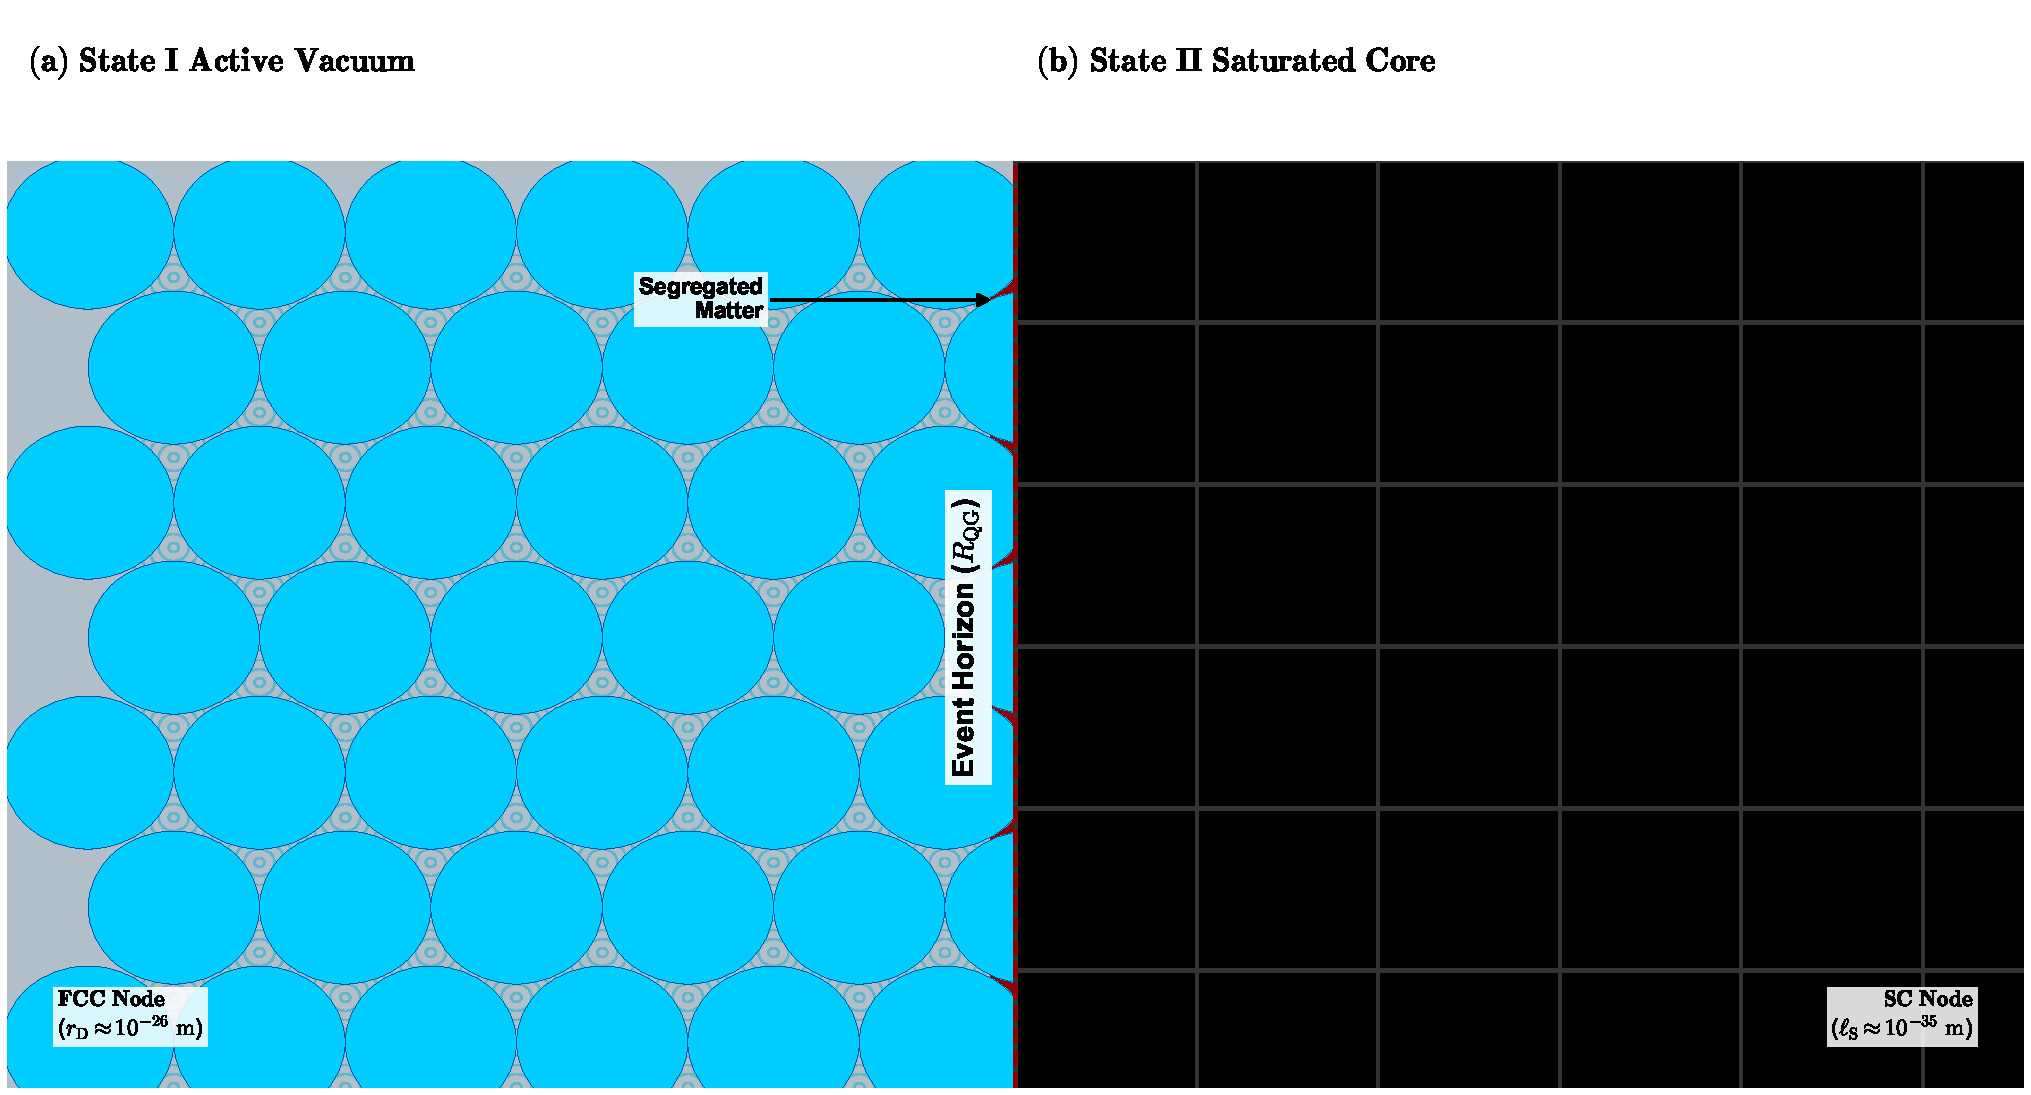
\includegraphics[width=0.9\textwidth]{Fig10_PartII_FCCtoSCTransition.pdf}
    \caption{\textbf{The Vacuum Phase Transition (FCC $\rightarrow$ SC).} The Event Horizon ($R_{QG}$) is visualized not as a spatial hole, but as a macroscopic crystallization front driven by gravitational saturation ($\alpha_G = 1$). \textbf{(a) State I (Active Vacuum):} The dynamic Face-Centered Cubic (FCC) lattice provides the geometric tolerance (interstitial voids) required for mass-energy. This structural flexibility permits ordered pilot-wave vibration (concentric ripples) and the active flow of time ($t > 0$). \textbf{(b) State II (Saturated Core):} As the boundary advances, critical gravitational strain forces the nodes into a strict Simple Cubic (SC) lock. This structural phase transition back to the substrate floor completely eliminates the voids, mechanically arresting all field oscillation and freezing the core into a static, fully packed, timeless block ($t = 0$).}
    \label{fig:fcc_sc_transition}
\end{figure}

\section{The Microphysics of Collapse: From Matter to Substrate}
The formation of this Substrate Core follows a precise mechanical sequence, governed by the density hierarchy derived in \hyperref[app:phase_transition]{Appendix \ref*{app:phase_transition}}. It is a process of stripping away the geometric conditions required for vibration.

\begin{itemize}
    \item \textbf{Deconfinement (The Neutron Breakdown):} As gravitational pressure exceeds Strong Force tension, neutrons are mechanically crushed. They dissolve into a quark-gluon plasma of fundamental knots ($r_D$).
    \item \textbf{Vibrational Saturation ($\rho_Q$):} As the plasma densifies, the vibrational velocity of these fundamental knots approaches the speed of light. The system reaches the Quantum Saturation Density ($\rho_Q \approx 9.07 \times 10^{61} \text{ kg/m}^3$). The lattice voids are energetically saturated, but the FCC geometry remains intact.
    \item \textbf{Geometric Locking ($\rho_{QG}$):} Gravity forces the knots to pack ``shoulder-to-shoulder.'' When the density reaches the Convergence Density ($\rho_{QG} \approx 4.43 \times 10^{70} \text{ kg/m}^3$), the Interstitial Voids (the empty space in the FCC lattice required for oscillation) are exhausted.
    \item \textbf{The Phase Transition (FCC $\rightarrow$ SC):} To resolve the topological stress of ``zero void'' packing, the lattice undergoes a martensitic transformation. The FCC geometry snaps into the Simple Cubic (SC) configuration.
        \begin{itemize}
            \item \textit{Mechanism:} The packing factor jumps discontinuously from $0.74$ to $1.0$.
            \item \textit{Result:} The voids vanish. Without voids, vibration is mechanically impossible. The ``Matter'' (dynamic wave) becomes ``Substrate'' (static stress).
        \end{itemize}
\end{itemize}

\section{Merging with the Substrate: The Scale Collapse}
Once the geometric voids are saturated at $\rho_{QG}$, the lattice loses the vibrational pressure that maintains the Duality Radius ($r_D$). The ``Inactive Soft Floor'' is unstable. The system undergoes a structural Scale Collapse, causing the macroscopic $r_D$ scaffolding ($\approx 7.89 \times 10^{-27} \text{ m}$) to dissolve directly into the underlying Substrate ($\ell_S \approx 10^{-35} \text{ m}$).

Consequently, the core density does not stop at the trigger point ($\rho_{QG} \approx 4.43 \times 10^{70} \text{ kg/m}^3$). Instead, it undergoes a discontinuous Density Jump to the Substrate Limit ($\rho_S \approx 5.15 \times 10^{96} \text{ kg/m}^3$), as detailed in \hyperref[app:phase_transition]{Appendix \ref*{app:phase_transition}}.

The Black Hole core is therefore the end of gravity. Because the core is a 100\% packed solid, it is strictly incompressible. An incompressible medium cannot support a density gradient. Therefore, since the system reaches the maximum tension field limit with a zero tension-gradient ($\nabla\tau = 0$), gravity---which is defined as a gradient---ceases to exist within the core. The core is mechanically indistinguishable from the underlying Substrate that permeates the universe. The matter that fell in has effectively merged with the vacuum background, adding its potential energy to the global tension of the field.

\begin{figure}[H]
    \centering
    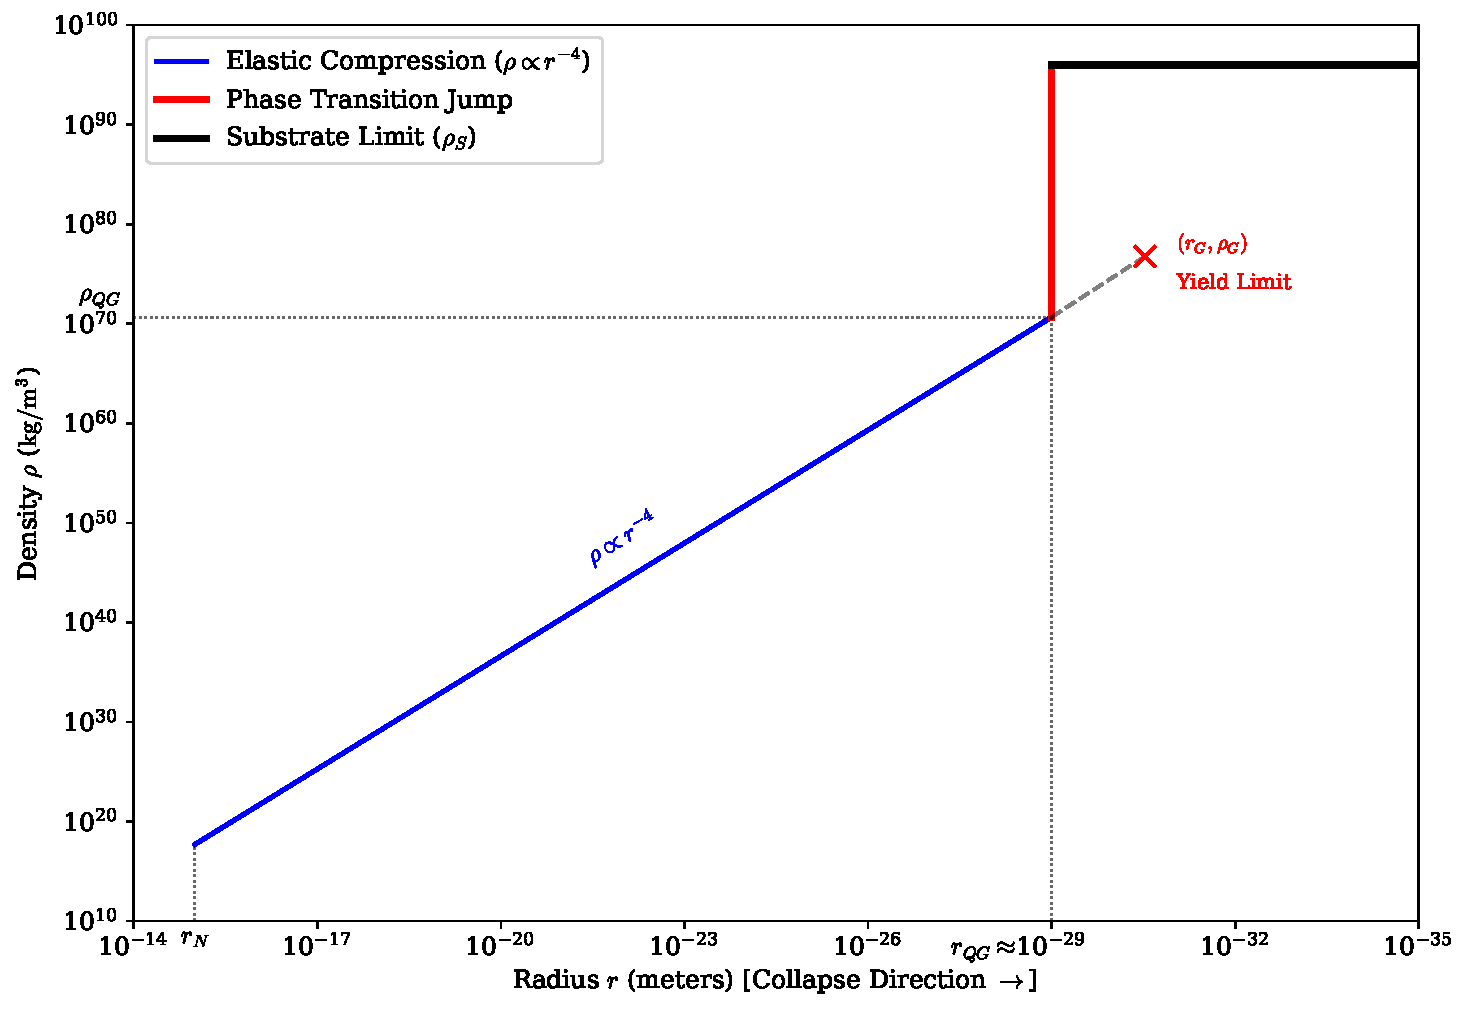
\includegraphics[width=0.9\textwidth]{Fig11_PartII_PhaseTransitionLogLog.pdf}
    \caption{\textbf{Gravitational Saturation and the Vacuum Phase Transition.} This log--log plot illustrates the mechanical response of the vacuum lattice during continuous gravitational contraction. \textbf{Elastic Compression (Blue Line):} Starting from the nucleon scale ($r_N$), as the local radius decreases, the field density rises according to the vacuum geometric scaling law ($\rho \propto r^{-4}$). \textbf{Void Exhaustion ($r_{QG} \approx 5.87 \times 10^{-29} \text{ m}$):} At the convergence density ($\rho_{QG} \approx 4.43 \times 10^{70} \text{ kg/m}^3$), the active interstitial voids are mechanically exhausted. The lattice reaches absolute gravitational saturation ($\alpha_G = 1$). \textbf{Phase Transition Jump (Red Line):} Instead of compressing further toward the structural yield limit where the space manifold would physically fracture (red "$\times$" at $\rho_G$), the system undergoes a discontinuous scale collapse. The core phase-shifts directly to the fundamental substrate density ($\rho_S \approx 5.15 \times 10^{96} \text{ kg/m}^3$), effectively resetting the localized volume to the static stability limit of the Hard Floor.}
    \label{fig:phase_transition_loglog}
\end{figure}

\section{The Resolution of the Information Paradox}
The Phase Transition model provides a direct mechanical resolution to the Information Paradox (the conflict between Unitarity and Hawking Radiation). As detailed in \hyperref[app:information_paradox]{Appendix \ref*{app:information_paradox}}, TFT distinguishes between Volumetric Storage and Holographic Access:

\begin{itemize}
    \item \textbf{Cold Storage (The Node Law):} Information is stored in the specific topological arrangement of the static SC lattice nodes within the core. Since the core is a solid crystal, its absolute information capacity scales with its Volume ($S_{\text{core}} \propto V$). The physical information is preserved in ``deep freeze.''
    \item \textbf{Surface Projection (The Holographic Law):} The Event Horizon acts as a phase boundary that screens the interior. To an outside observer, the measurable information accessible via field strain is limited to the surface area of the boundary ($S_{\text{obs}} \propto A$).
\end{itemize}

\textbf{The Solution:} Information is never destroyed; it is topologically locked. The paradox arises only when standard models mistakenly assume the observable surface entropy (Area) represents the total physical content. In TFT, the surface entropy is merely the ``Index'' of the library, while the books themselves remain entirely intact within the frozen SC volume.

\section{The Black Hole Horizon and Causality}
In Part I, we established that inertial mass arises from the hydrodynamic drag of the lattice condensate. We further defined the lattice kinematic budget as $c_E^2$, representing the invariant energy cost of the vacuum structure. Therefore, the propagation speed of any causal signal ($c_P$) is governed by the ratio of this invariant potential to the effective inertia ($\mu_{\text{eff}}$) of the local medium:
\begin{equation}
    c_P = c_E \sqrt{\frac{\mu_D}{\mu_{\text{eff}}}} \cos(\Delta\phi)
\end{equation}

We define the effective inertia as a function of the dimensionless gravitational coupling:
\begin{equation}
    \alpha_G = \frac{GM}{r c_E^2}
\end{equation}
\begin{equation}
    \mu_{\text{eff}} = \frac{\mu_D}{(1 - \alpha_G)^4}
\end{equation}

\subsection*{The Black Hole Horizon}
As the gravitational potential approaches the vacuum budget ($\alpha_G \rightarrow 1$), the effective inertia diverges ($\mu_{\text{eff}} \rightarrow \infty$), and causal speed halts ($c_P \rightarrow 0$). Therefore, we define the Black Hole Horizon radius as $R_{QG} = \frac{GM}{c_E^2}$. This radius marks the exact geometric threshold of the FCC $\rightarrow$ SC phase transition, where the local density reaches the convergence limit ($\rho_{QG}$), as derived in \hyperref[app:phase_transition]{Appendix \ref*{app:phase_transition}}.

\textit{(Note: TFT predicts that at the standard Schwarzschild radius $R_s$, where $\alpha_G = 0.5$, the causal speed slows to $c_P \approx 0.25c_E$, meaning propagation remains physically possible).}

\subsection*{The Three Limits of Causality}
From the mechanics of the lattice, we distinguish three fundamental modes by which causality is constrained:

\begin{description}
    \item[\textbf{Type I: Gravitational Causal Failure (Black Hole)}] \mbox{}
    \begin{itemize}
        \item \textbf{Mechanism:} Inertial Saturation (Density Limit).
        \item \textbf{Physics:} The local inertial density increases due to macroscopic mass concentration until the lattice mechanically fails. Light propagation ($c_P$) ceases because the node becomes phase-locked into the rigid substrate.
        \item \textbf{State:} Phase transition (FCC $\rightarrow$ SC).
        \item \textbf{Definition:} A mechanical rupture of the active spacetime medium due to extreme background tension.
    \end{itemize}
    \vspace{0.3cm}

    \item[\textbf{Type II: Cosmological Causal Saturation (Cosmic Horizon)}] \mbox{}
    \begin{itemize}
        \item \textbf{Mechanism:} Cumulative Drag (Distance/Energy Exhaustion).
        \item \textbf{Physics:} The average inertial density remains low and the lattice remains intact (FCC). However, the integrated gravitational potential over the macroscopic cosmic radius ($R_U$) exhausts the lattice energy budget: $\phi_{G,U} = \int_0^{R_U} \frac{G \cdot dm}{r} = c_E^2$
        \item \textbf{State:} Phase equilibrium. The medium is intact, but cumulative thermodynamic drag prevents further information transfer.
        \item \textbf{Definition:} A visibility limit where the energetic cost of propagation equals the energy of the wave.
    \end{itemize}
    \vspace{0.3cm}

    \item[\textbf{Type III: Kinematic Causal Failure (The Nyquist Limit)}] \mbox{}
    \begin{itemize}
        \item \textbf{Mechanism:} Kinematic Saturation (The Quantum Energy Limit).
        \item \textbf{Physics:} Causality can fail even in the active vacuum if a single transverse wave becomes too energetic. In solid-state mechanics, the Nyquist limit dictates that a wave cannot propagate if its wavelength is physically shorter than the nodes of the medium. Setting the minimum wavelength to the fundamental lattice node radius ($\lambda_{\text{min}} = r_D \approx 7.89 \times 10^{-27} \text{ m}$) defines the Quantum Energy Limit ($E_Q$): $E_Q = \frac{h c_E}{r_D} \approx 25.18 \text{ Joules} \approx 1.57 \times 10^{11} \text{ GeV}$
        \item \textbf{State:} Localized Phase Transition. If a localized event attempts to inject a photon exceeding this limit, the structural tension physically surpasses the kinematic capacity of the Soft Floor. Frequency scaling becomes mechanically impossible.
        \item \textbf{Definition:} An absolute kinematic energy ceiling for a single wave, completely preventing the ``ultraviolet catastrophes'' and infinite energies of standard quantum mechanics by forcing a localized phase transition.
    \end{itemize}
\end{description}

\subsection*{Conclusion}
The boundaries of the observable universe are strictly dictated by the mechanical capacity of the FCC lattice:
\begin{itemize}
    \item \textbf{A Black Hole (Type I):} A region where the background medium reaches gravitational saturation ($\rho_{QG}$) and structurally locks.
    \item \textbf{The Cosmic Horizon (Type II):} A boundary where a signal exhausts its energy to acoustic drag over a macroscopic distance.
    \item \textbf{The Nyquist Limit (Type III):} A localized threshold where a signal forces a phase transition due to a frequency exceeding the geometric resolution of the vacuum.
\end{itemize}